
\cleardoublepage


\chapter{Experimental Validation}


% introduction here
% ----------------------------------------------------------------------------


\section{Modeling}

\subsection{NEBP Decoupling}

% why model?
Before conducting any flux measurement of the beam port, the experimental setups were first modeled in MCNP.
The purpose of this is twofold: one, this generates predicted detector responses to aid in the selection of experimental parameters and give an idea for the physicality of initially obtained results, and two, response functions are generated that are ultimately used in the unfolding of the final spectrum.
% can i use the full model?
However, due to the (computational) size of the full reactor model, it would be very expensive to generate these experimental responses and response functions.
Also, the beam port flux, not in-core source spectrum is what we desire to measure, so the response functions would not be properly generated using the full model in this analysis.
% no, we need a decoupled model
Necessarily, a decoupled model of the beam and experimental configurations must be used for this portion of the simulation.
This will simplify the geometry and transport significantly, allowing for reduced computation times and also for the ultimate unfolding of the correct neutron spectrum.
% is it valid to decouple?
As to the validity of this decoupling, as long as the full surface current leaving the outer boundary of the full model is captured in the decoupled model, then this approach is neutronically equivalent to a non-decoupled approach.
% yeah, as long as the coupled surfaces capture the outgoing flux, in our case that's justified because a vast majority comes down the beam
In our case, as indicated by the flux results from the previous chapter, the majority of departing neutrons leave the beam through the collimator void.
The tallies include a large area around this beam, too, to account for any neutrons that excape the beam.
This flux value decreases rapidly further from the center of the beam, and so it is believed that any neutrons that escape the collimator, leave through the structural material around the collimator, and still manage to interact in any detector will contribute in a statistically insignificant way.

% what does the decoupled model include?
The decoupled model includes the 8" outer portion of the NEBP, which would account for any backscattering from either detector.
% well, i converted the tally into a source at the surface 
The tally from the full model was converted into a steady-state source placed at the outer face of the NEBP.
% the beam and space outside contain universes that different detectors can be included in
The collimator void and space outside of the NEBP contain universes that allow different detectors to be swapped in and out of the model.
% the whole thing is wrapped and driven by python, too so that's great
The entire decoupled model is wrapped in python to allow for variation in input parameters and for the easy extraction and processing of output data.


\subsection{Gold Foil Tube}

% the foil tube was a type of spectrometer
The gold foil tube is a kind of neutron spectrometer.
% the gold foil tube design was based on the bonner sphere - thermal responsing detector with varying moderation
In design, it is principally based on the bonner sphere spectrometer.
Gold foils, which preferentially absorb thermal neutrons are spaced with sections of high density polyethylene (HDPE).
% produce independent responses
HDPE is a strong neutron moderator, meaning that the response of each foil will be somewhat independent of the others, since neutrons are slowing down and being absorbed between foils.
% it was also meant to help with beam alignment and to simplify the beam characterization process
This design also is advantageous in that it solves issues with beam alignment and only requires a single irradiation to generate multiple responses.

%
%\begin{figure}[htb]
%\centering
%\includegraphics[height=4in]{tex/figures/.png}
%\caption[]{}
%\label{fig:}
%\end{figure}


% you can see the device in FIG
The gold foil device can be seen in FIG.
% there are three major components, the aluminum tube, the hdpe separators and the gold foils
The tube is comprised of three separate materials, the gold foils, the HDPE separators, and the aluminum containment tube.
% the gold foils are __ diameter and __ thickness
Each of the gold foils are 5$mm$ in diameter and 0.1$mm$ thick.
% the hdpe was cylinders of __ size
The HDPE sections were 1" thick cylinders.
% each hdpe piece had a __ size hole drilled into it where the gold foil would be situated
A 1$mm$ depth, 5$mm$ OD hole was drilled into the front of each section where the gold foil was situated.
% all of these would be encased in __ID __OD aluminum tubing
All of these sections were sandwiched together and encased in 0.75" OD, 1/24" thick aluminum tubing.
% aluminum is chosen because it's relative insensitivity towards neutrons
Aluminum was chosen because of its relative insensitivity to neutrons.
% the whole apparatus had __ hdpe pieces and foils, with the first foil being exposed and a gap of __ at the beginning
The whole apparatus was comprised of 12 HDPE pieces and foils, with the first, exposed foil being situated 1" from the start of the tubing.

% this device was modeled in mcnp, where f4 flux tallies, folded with the au n,g response were used with a scx card to produce the rfs
This device was modeled in MCNP, where f4 flux tallies, folded with the $^{198}$Au(n,$\gamma$) cross sections were used with an SCX card to produce the response functions.

\subsection{Bonner Sphere Spectrometer}

% a second, active detector was included in the experiment, too, the bss
% the bonner sphere spectrometer uses a series of plastic spheres surrounding a lithium iodide detector to produce independent responses

%
%\begin{figure}[htb]
%\centering
%\includegraphics[height=4in]{tex/figures/.png}
%\caption[]{}
%\label{fig:}
%\end{figure}



% you can see the device in FIG
% the full device was modeled using the 4x4 mm detection crystal coupled with pmt and hdpe sphere
% positioned a distance of __ from the bp aperture
% rfs were generated for sphere sizes of __ __ __ whatver
% the tally used f4 folded with the n,t reaction in the crystal with the scx card again



\subsection{Response Functions}

% describe any post processing used for these results to get the values in cm2

% add the plots and then discuss

% the gold foil tube response functions
\begin{figure}[htb]
\centering
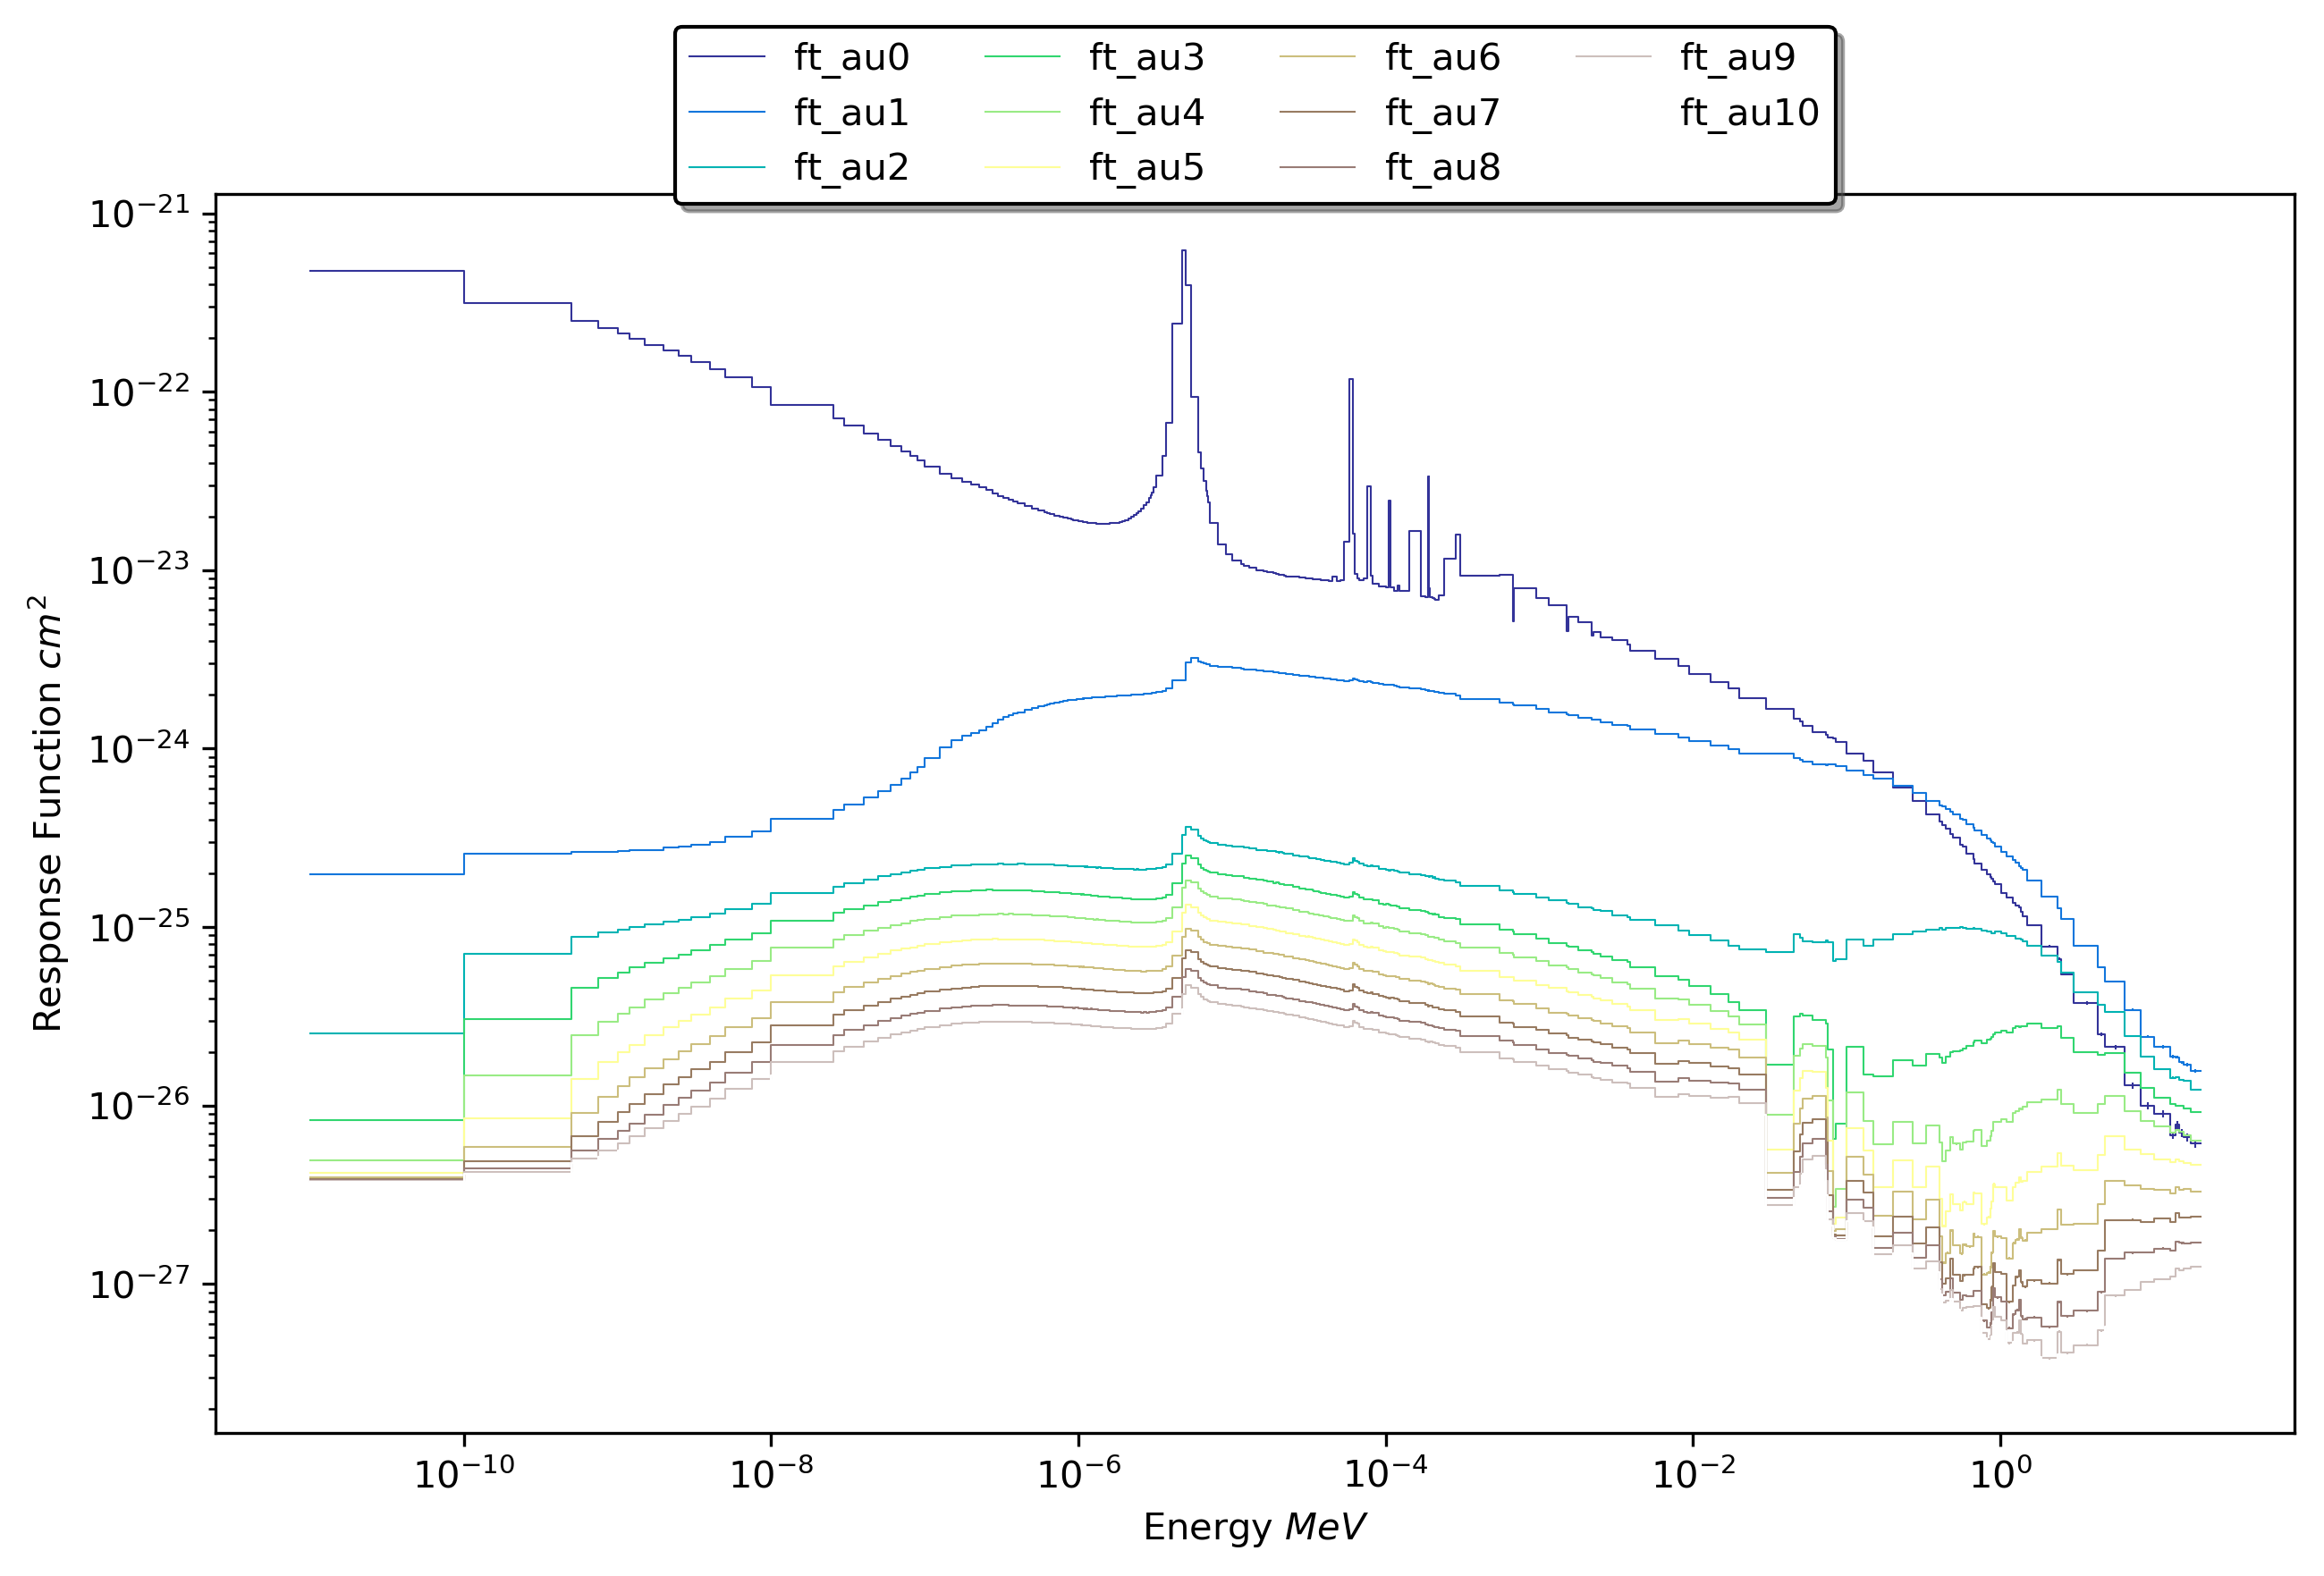
\includegraphics[height=4in]{tex/figures/ft_au.png}
\caption[Gold Foil Tube Response Functions]{The response functions for the gold foil tube.}
\label{fig:ft_au_rfs}
\end{figure}

% discuss the ft_au response functions

% the bonner sphere response functions
\begin{figure}[htb]
\centering
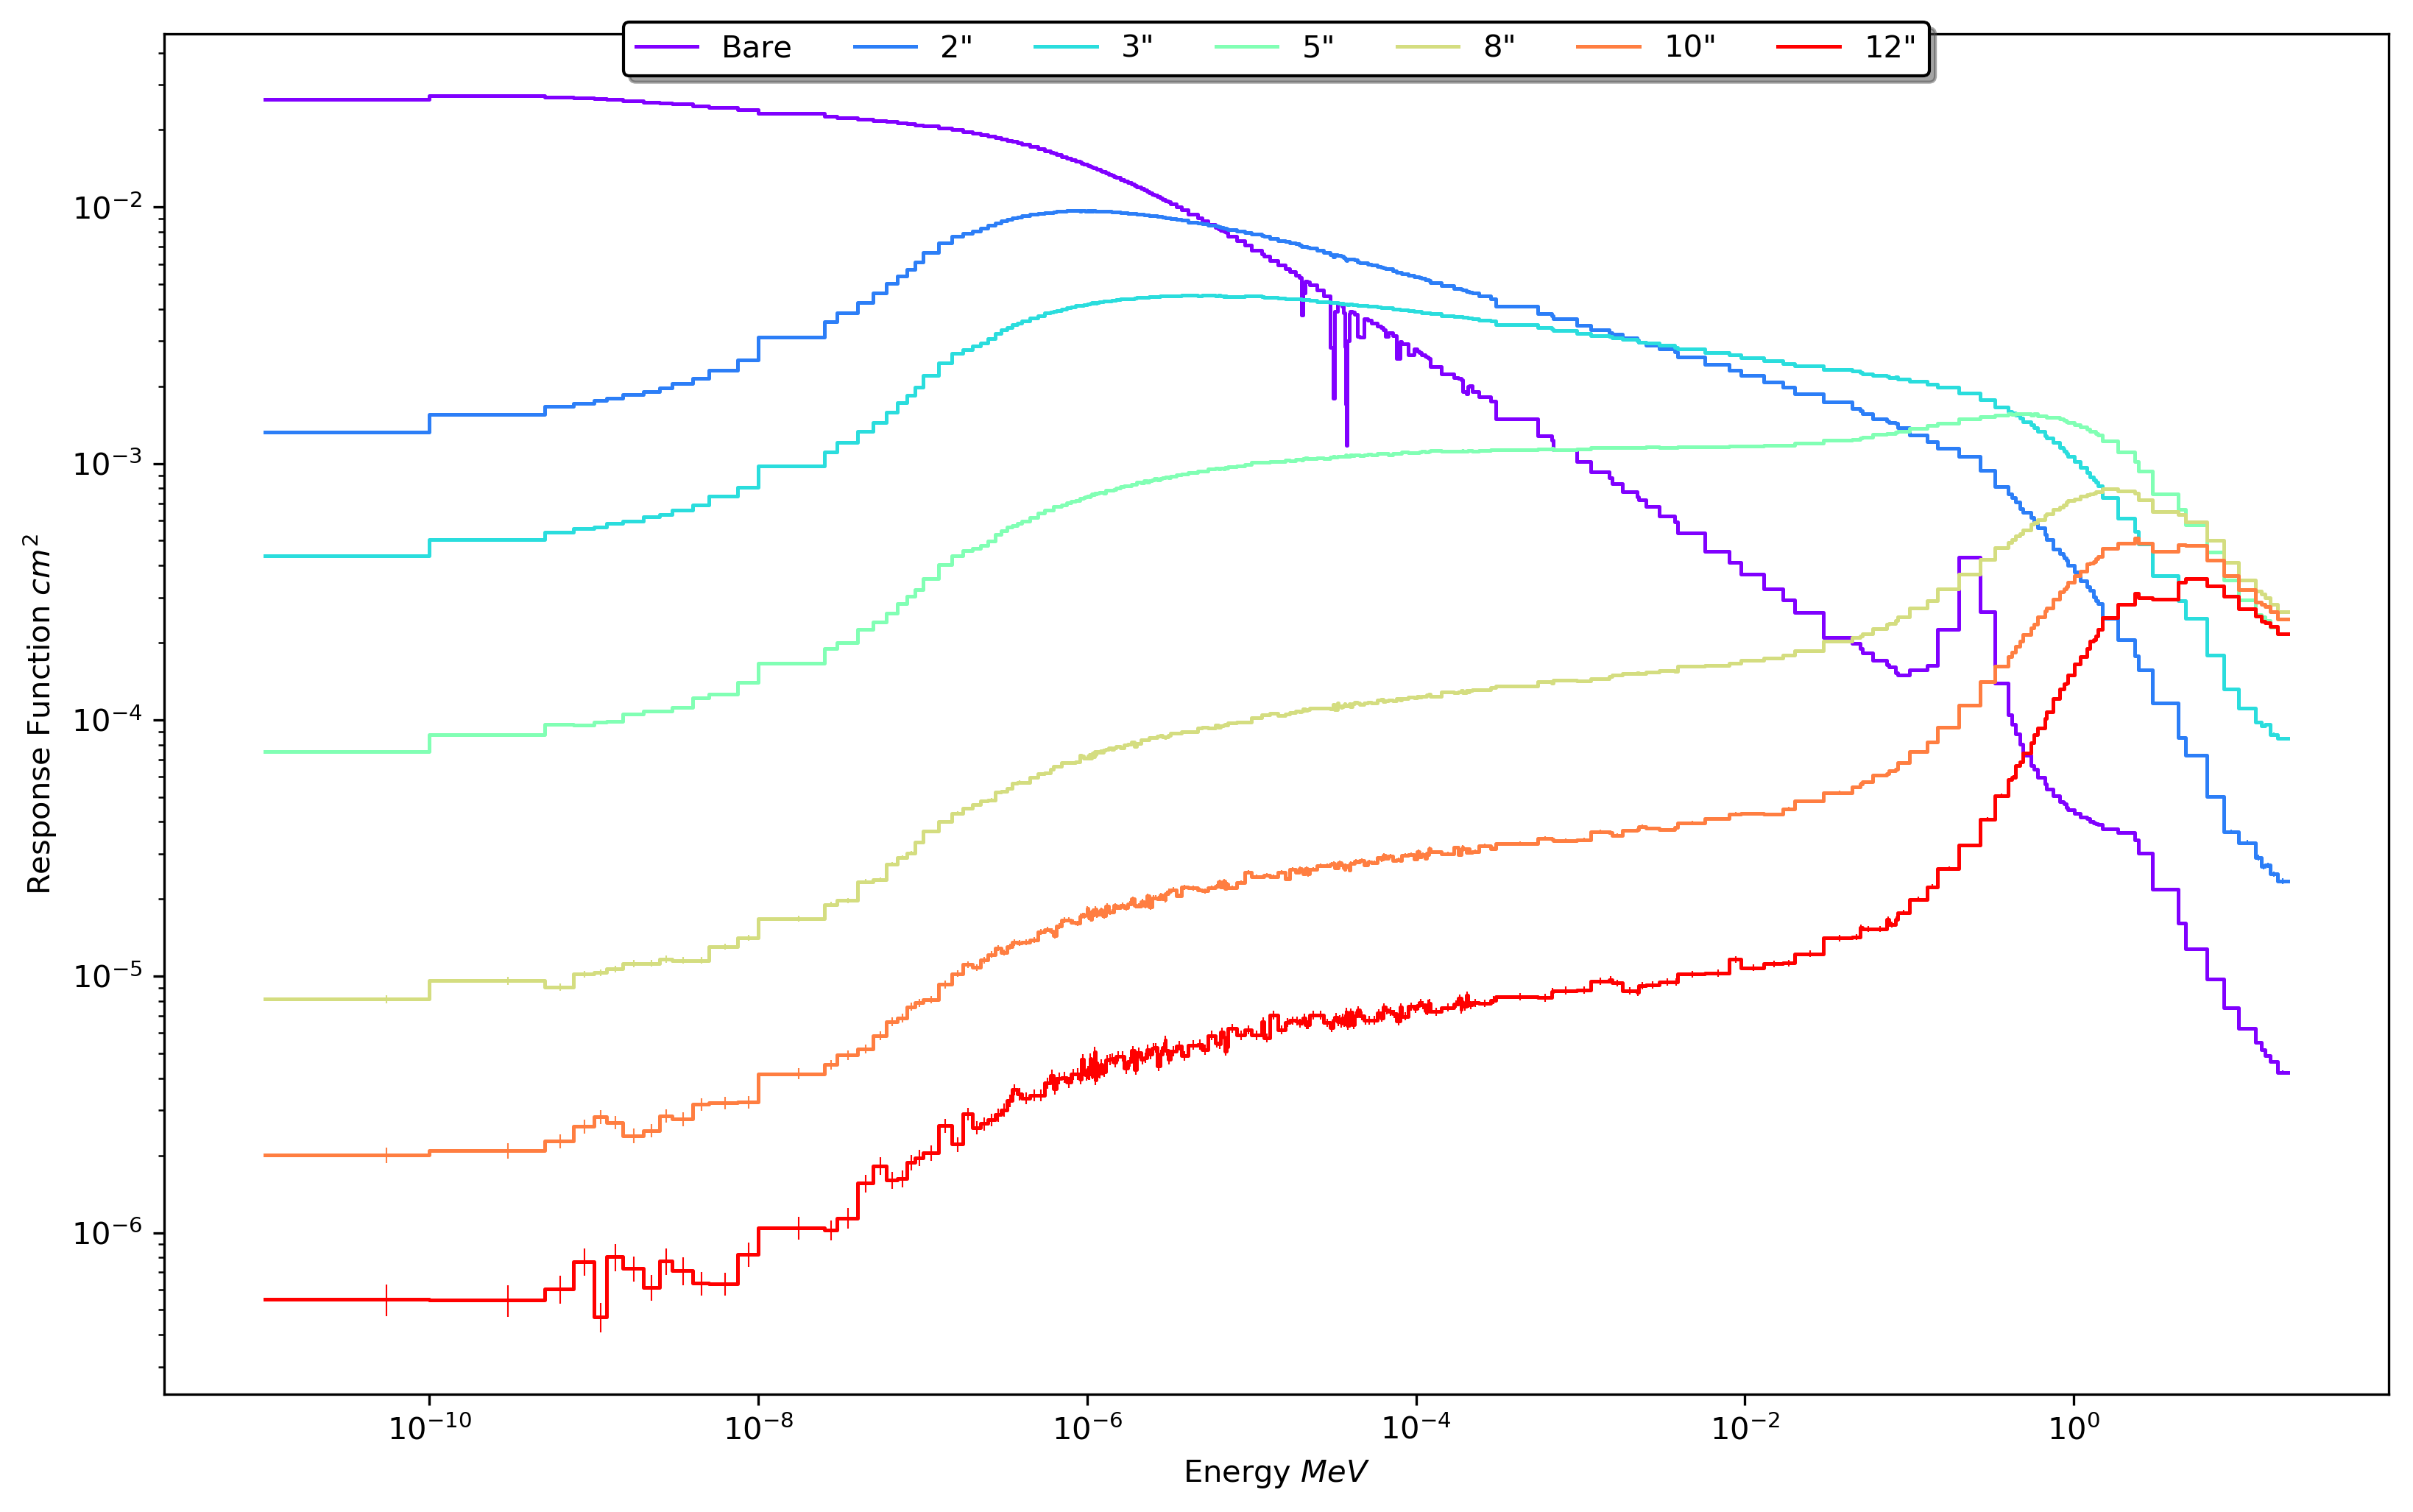
\includegraphics[height=4in]{tex/figures/bs.png}
\caption[Bonner Sphere Spectrometer Response Functions]{The response functions for the Bonner Sphere Spectrometer.}
\label{fig:bs_rfs}
\end{figure}

% discuss the bss response functions

% ----------------------------------------------------------------------------
% other stuff here
